\emph{Pregunta 11.1}
\emph{¿Cuantas señales están definidas en su sistema?}
\\
38 señales en total
\\

\emph{¿Cuales solo detienen el proceso?}
\\
SIGSTOP (17, 19, 23)\\
SIGTSTP (18, 20, 24)\\
SIGTTIN (21, 26)\\
SIGTTOU (22, 27)\\
\\

\emph{¿Cuáles señales no pueden ser capturadas?}
\\
SIGKILL (9) y SIGSTOP (17, 19, 23)
\\

\emph{Programa 11-1}
\centerline{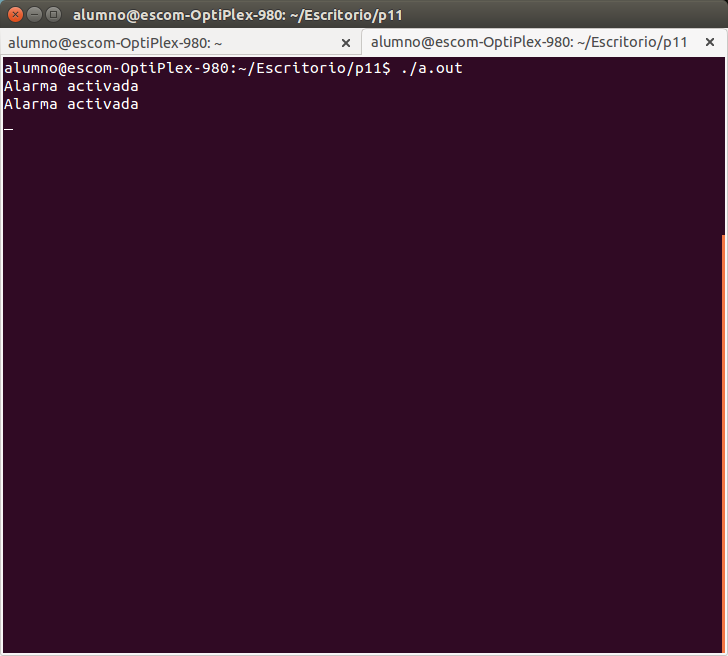
\includegraphics{img/s1}}
\

\emph{Ejercicio 11.1}
\\
\emph{Modifique el programa para que se envíe la señal SIGALARM cada medio segundo en lugar de cada 3:}
\begin{lstlisting}

ualarm(500000, 0);

\end{lstlisting}
\emph{Modifique la función manejadora de señal para que imprima el número de señal que le envía el kernel}
\\
El código:
\\
\begin{lstlisting}

void tratar_alarma(int signum){
    printf("Alarma activada\n");
    printf("Numero de señal: %d\n", signum);
}

\end{lstlisting}
muestra que, efectivamente, es la señal 14 la recibida:
\\
\centerline\includegraphics{img/s2}}

\emph{Pregunta 11-2}
\\
\emph{Envíe la señal SIGALARM con el comando kill desde otra terminal y observe lo que pasa}
\\
Al enviarla de esa manera, la impresión se realizará aunque no haya transcurrido el tiempo especificado en alarm() o ualarm() pues el programa la recibe en cuando la mandamos.
\\
\emph{¿Qué pasa si añade SIGALARM a la máscara?}
\\
\begin{lstlisting}

sigaddset(&mask, SIGALRM);

\end{lstlisting}
El proceso nunca hará una impresión pues la señal siempre será ignorada.
\\

\emph{Pregunta 11.3}
\\
\emph{¿Cuál es la línea que se ejecuta inmediatamente después de ejecutarse el manejador de señales?}
\\
Línea 6 (declaración del temporizador al inicio del ciclo for)